\documentclass{book}

\usepackage[utf8]{inputenc}
\usepackage[T1]{fontenc}
\usepackage[francais]{babel}
\usepackage{graphicx} 
\usepackage{adjustbox}
\usepackage{fancyref}
\usepackage{hyperref}
\usepackage{url}


\title{%
  Projet de Sciences des Données \\
  \large Explotation d'images satellites haute-résolution \\pour la prévision d'indicateurs socio-économiques \\
    }

\author{\textsc{Youcef} - \textsc{Kacer}}
\date{22 Septembre 2016}

\begin{document}
 
\maketitle

\tableofcontents

\frontmatter
\chapter{Introduction}
Ce document a pour but de présenter le procédé de géoréférencement d'images. Concrètement, il s'agit de donner aux points 
d'une image quelconque rectangulaire de prise de vue aérienne, des coordonnées géographiques dans un certain système de coordonnées
via une transformation géométrique.
En effet, un point de l'image de départ, est simplement répéré par ses coordonnées de ligne et de colonne mais n'a aucune caractéristique
géographique.\\
Nous allons appliquer cela en utilisant le $SIG$ open-source $QGIS$ sur $Ubuntu$. Plus précisemment, l'exemple traité aura pour but de
vérifier la fiabilité des images géoréférencées du satellite \begin{itshape}LANDSAT-8\end{itshape}.

\mainmatter
\chapter{Géoréférencement d'images aériennes}
\section{Principe}\label{principe_geo}

Une première méthode pour le géoréférencement d'une image dans un certain système de coordonnées, nécessite la connaissance 
des coordonnées d'un 
certain nombre de points de l'image dans ce système de coordonnées, ce sont les \begin{itshape}points d'amers\end{itshape}.
A partir de ces points, une transformation d'un certain ordre est appliquée aux autres points de l'image afin de leur attribuer 
des coordonnées dans ce système.\\
Les images de prise de vue aérienne peuvent être livrées déjà géoréférencées dans un certain système de coordonnées géographiques, 
c'est le niveau 2 de rectification dans la nomenclature du cours de Jean-Marie Nicolas \cite{Nicolas:2014}.\\

\section{Les systèmes de géoréférencement}

Il en existe une multitude dont le nom est codifié par l'\begin{itshape}European Petroleum Survey Group\end{itshape} depuis 1985.\\
A titre d'exemple, l'$IGN$ (\begin{itshape}Institut Géographique National\end{itshape}) géoréférence ces images via plusieurs
systèmes de géoréférencement possibles dont:\\

\begin{itemize}

\item[-] \begin{itshape}NTF 93/Lambert 93\end{itshape} dont le code est \begin{itshape}EPSG:2154\end{itshape}.\\
\item[-] \begin{itshape}NTF Paris/Lambert zone II étendu\end{itshape} dont le code est \begin{itshape}EPSG:27572\end{itshape}.\\
 
\end{itemize}

Les images du satellite \begin{itshape}Landsat-8\end{itshape} sont géoréférencées dans le système 
\begin{itshape}WGS84/Mercator\end{itshape} dont le code $EPSG$ dépend
de la zone $UTM$ (\begin{itshape}Universe Transverse Mercator\end{itshape}) où l'on se situe dans le globe 
(par exemple \begin{itshape}EPSG:32631\end{itshape} pour la zone \begin{itshape}UTM\end{itshape} $31N$ contenant la commune de
 \begin{itshape}Thonon-Les-Bains\end{itshape}).\\ 
Dans la section qui suit, nous proposons une méthode pour vérifier la fiabilité du géoréférencement
 des images du satellite \begin{itshape}LANDSAT-8\end{itshape}.
 
\section{Géoréférencement des images Landsat-8}

le site de l'$USGS$ (\begin{itshape}U.S. Geological Survey\end{itshape}) \cite{landsat8} qui met à disposition les images
satellitaires de \begin{itshape}LANDSAT-8\end{itshape}, ne précise pas la méthode utilisée pour leur géoréférencement.
Mais on peut toutefois vérifier sa fiabilité en comparant une image de ce satellite avec une image de 
l'$IGN$.\\
En effet, il suffirait de récupérer une image d'une certaine zone au format \begin{itshape}GeoTIFF\end{itshape}, 
donc géoréférencé, de l'$IGN$ et de la superposer
à une image \begin{itshape}LANDSAT-8\end{itshape} contenant la même zone. Toutefois, le géoréférencement de l'image $IGN$ étant différent
de celui de l'image \begin{itshape}LANDSAT-8\end{itshape}, il faudrait afficher la première dans le géoréférencement de la seconde.\\
Seulement, le site de l'$IGN$ ne propose des images géoréférencées qu'à l'achat, mais nous pouvons contourner cela en récupérant une 
image non géoréférencé, qu'on géoréférencerait ensuite via un logiciel $SIG$, $QGIS$ en l'occurence.\\

\subsection{Géoréférencement d'une image de l'IGN}

Le portail de l'IGN \cite{ign-portail} permet de parcourir le globe en affichant instantanément les coordonnées des points dans 
plusieurs systèmes de coordonnées possibles. La figure \ref{ign-portail} montre l'interface du portail affichant la commune de
\begin{itshape}Thonon-Les-Bains\end{itshape} en coordonnées \begin{itshape}NTF 93/Lambert 93\end{itshape}.

\begin{figure}[H]
\begin{center}
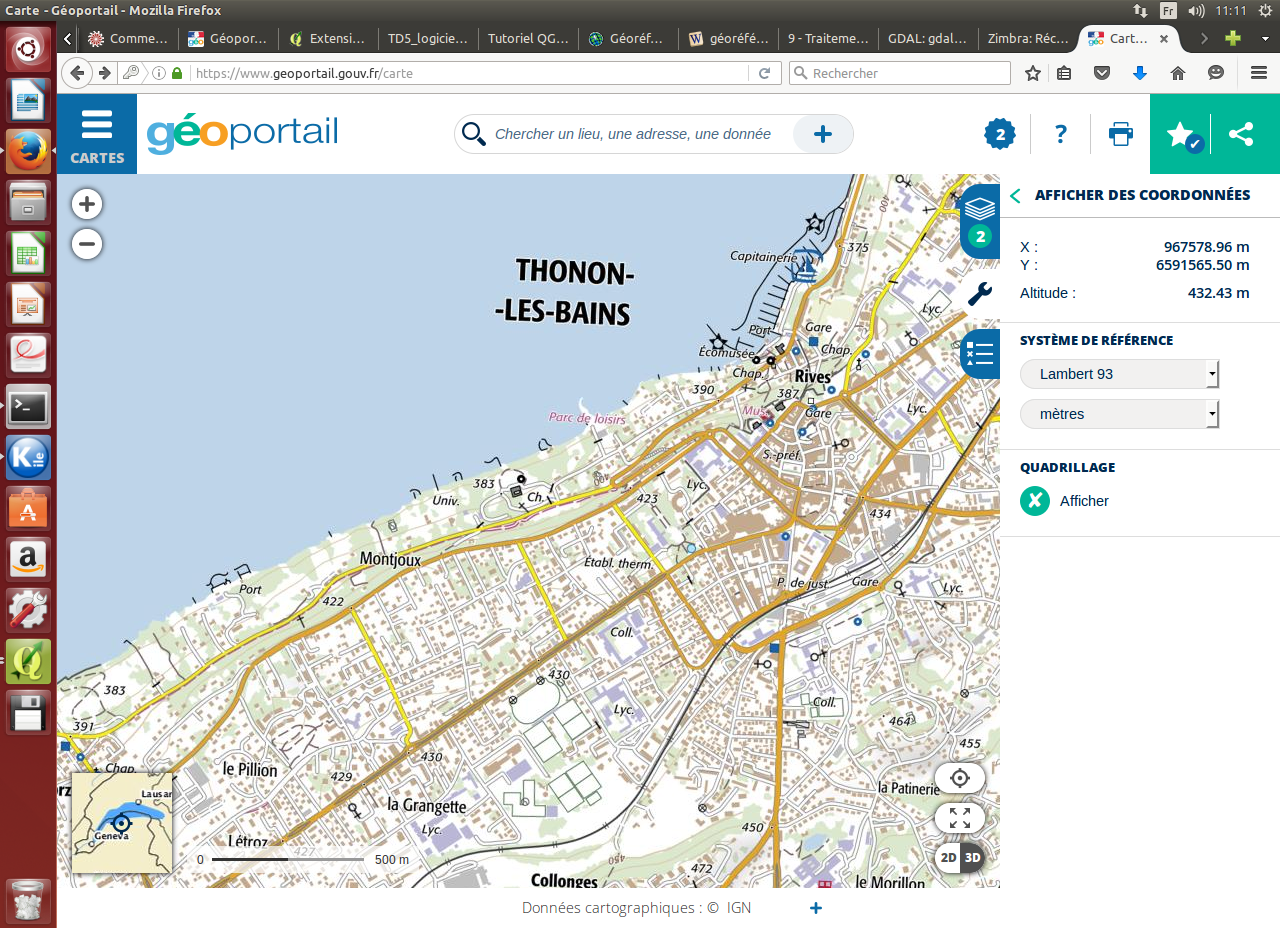
\includegraphics[scale=0.3]{images/ign-portail-Thonon.png}
\end{center}
\caption{portail de l'$IGN$ - commune de Thonon-Les-Bains en coordonnées NTF93/Lambert93 \cite{ign-portail}}
\label{ign-portail}
\end{figure}

\clearpage

La manipulation consiste à prendre un snapshot du portail pour cette zone, en affichant au préalable les coordonnées de 
plusieurs points via l'outil de marquage et d'annotation du portail. La figure \ref{ign-points} montre ainsi six points 
dont on a indiqué les coordonnées en \begin{itshape}NTF 93/Lambert 93\end{itshape}. Ces points vont jouer le rôle des 
\begin{itshape}points d'amers\end{itshape} décrits plus haut dans le principe de géoréférencement \ref{principe_geo}.

\begin{figure}[H]
\begin{center}
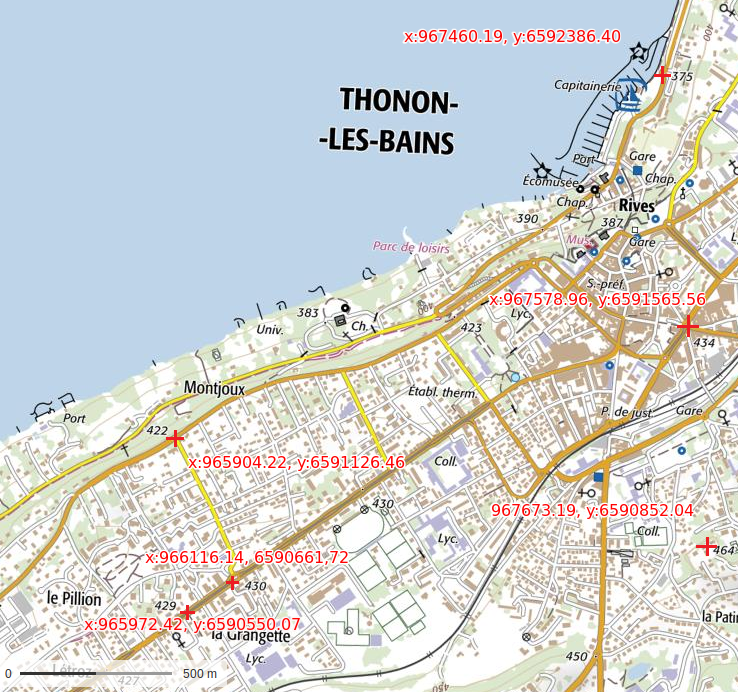
\includegraphics[scale=0.5]{images/ign-points-Thonon.png}
\end{center}
\caption{image non-géoréférencé de l'$IGN$ - commune de Thonon-Les-Bains et six points de contr\^{o}le en coordonnées NTF93/Lambert93}
\label{ign-points}
\end{figure}

\clearpage

Le logiciel libre $QGIS$ \cite{QGIS_software} permet de géoréférencer une image dans le même système de coordonnées que des points de
contr\^{o}le préalablement renseignés dans l'outil.\\
Pour commencer, il faut ouvrir un projet dans l'outil et renseigné le système de projection dans lesquel on souhaite visualiser
les images géoréférencées (on parle de \begin{itshape}raster\end{itshape}). On choisit ici le système de projection
\begin{itshape}EPSG:32631\end{itshape} car c'est celui dans lequel les images \begin{itshape}Landsat-8\end{itshape} sont projetées et
sur lequel on projetera notre snapshot IGN une fois géoréférencé, pour comparaison.\\
La figure \ref{qgis-projet} montre la manipulation dans les propriétés du projet.

\begin{figure}[H]
\begin{center}
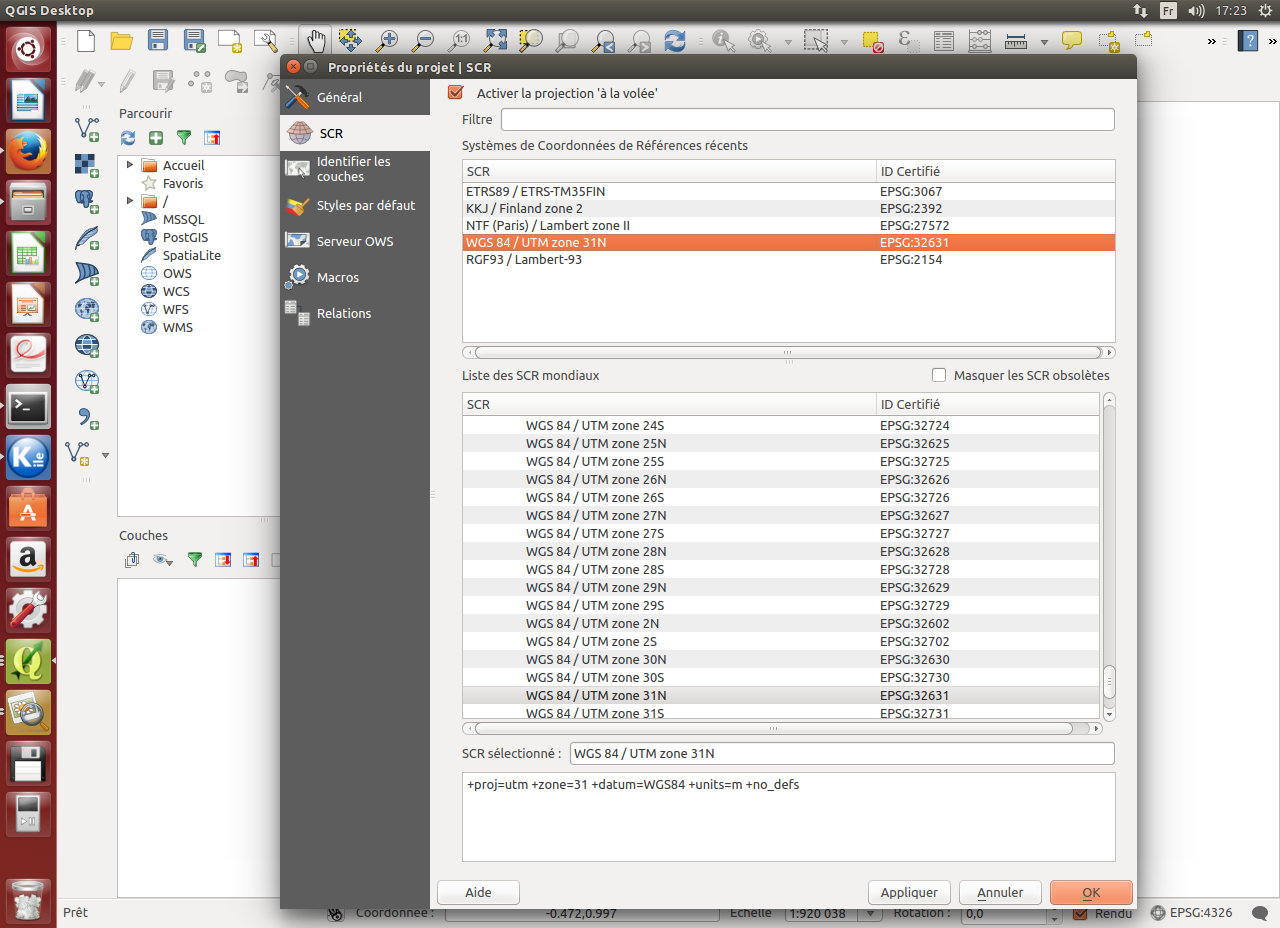
\includegraphics[scale=0.3]{images/qgis-projet.png}
\end{center}
\caption{Projet $QGIS$ et système de projection}
\label{qgis-projet}
\end{figure}

\clearpage

Ensuite, via l'onglet \og Raster > Géoréférencer > Géoréférencer\fg{}, on ouvre 
une nouvelle fen\^{e}tre dédiée au géoréférencement à partir de laquelle on charge notre snapshot \ref{qgis-georef} 
(onglet \og Ajouter un raster \fg{}).\\
L'outil demande alors de renseigner un système de projection pour le géoréférencement, on selectionne celui correspondant 
à nos points d'amers, soit \begin{itshape}NTF 93/Lambert 93\end{itshape} (\begin{itshape}EPSG:2154\end{itshape}).

\begin{figure}[H]
\begin{center}
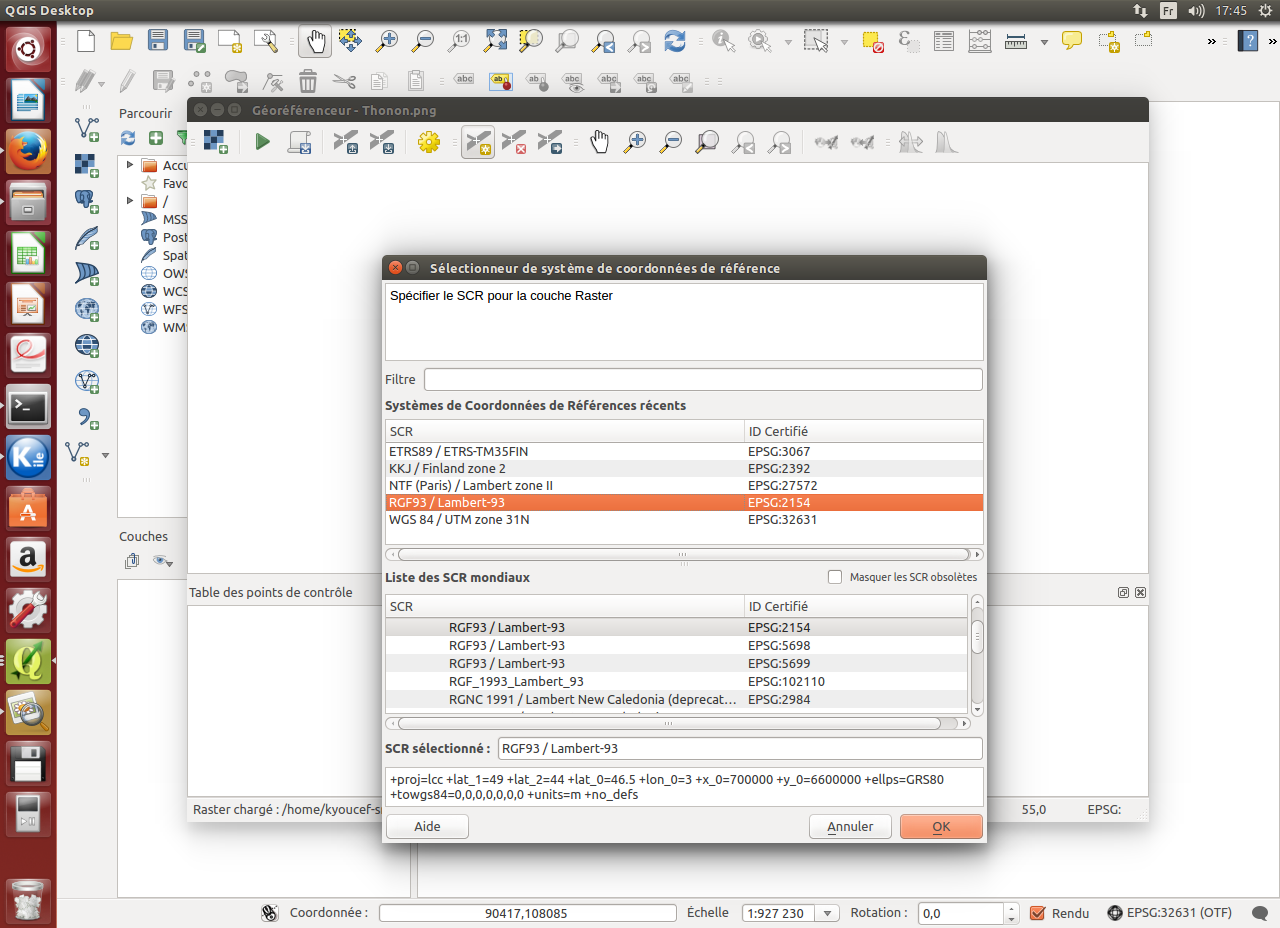
\includegraphics[scale=0.3]{images/qgis-georef.png}
\end{center}
\caption{Projet $QGIS$ et chargement d'une image non-géoréférencé pour géoréférencement}
\label{qgis-georef}
\end{figure}

\clearpage

Une fois le snapshot chargé, on renseigne les points de contr\^{o}le correspondant aux croix rouges sur le snapshot via l'onglet 
\og Ajouter un point \fg{}, dans la fenêtre de géoréférencement. On ajoute tour à tour les six points en renseignant
les coordonnées des points. La figure \ref{qgis-points} montre ainsi la fen\^{e}tre de géoréférencement contenant le snapshot 
et le tableau des points de contr\^{o}le en bas.

\begin{figure}[H]
\begin{center}
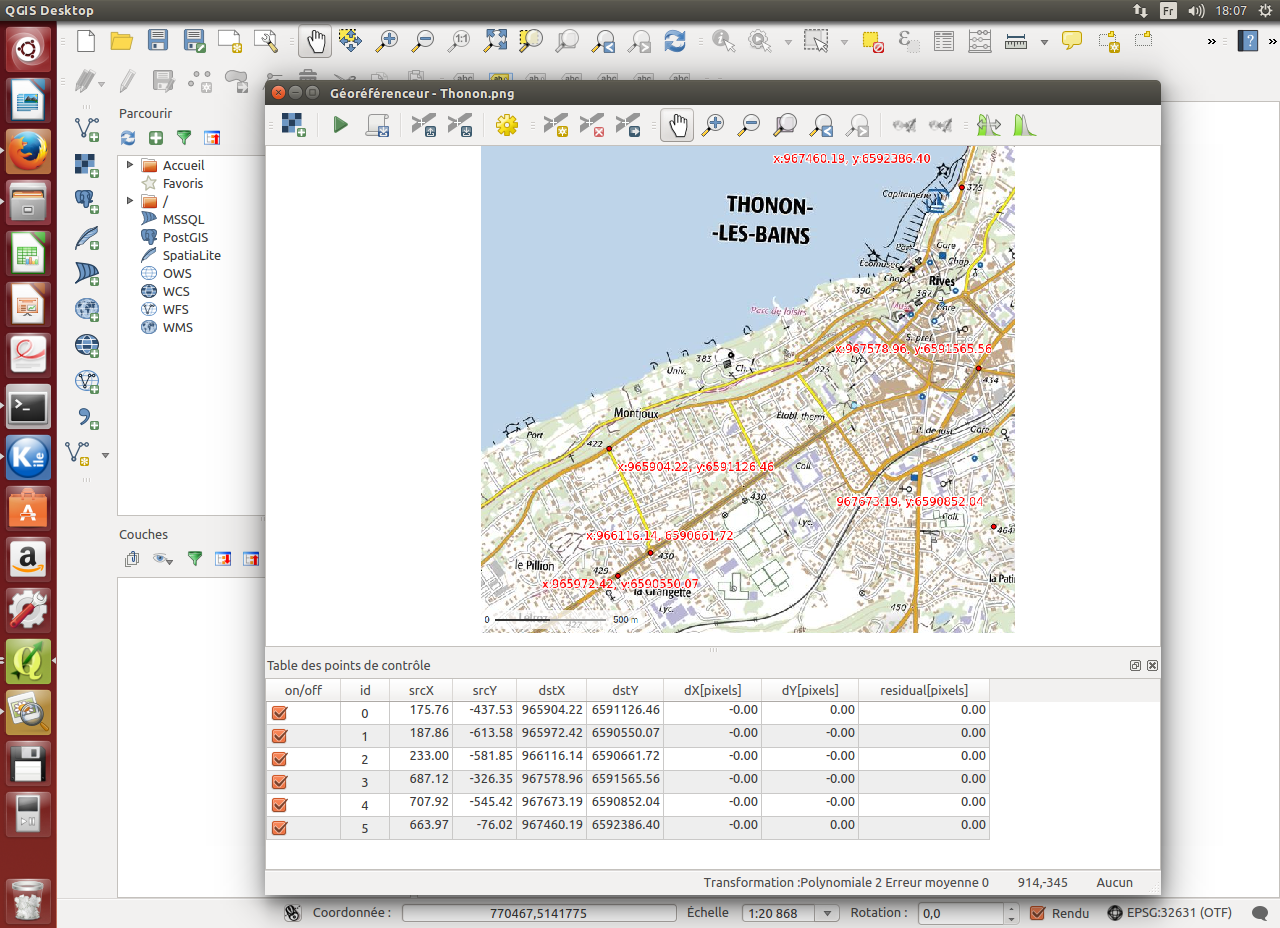
\includegraphics[scale=0.3]{images/qgis-points.png}
\end{center}
\caption{Projet $QGIS$ et renseignement des points de contr\^{o}le dans la fen\^{e}tre de géoréférencement}
\label{qgis-points}
\end{figure}

\clearpage

Maintenant que les points de renseignement sont données, on va définir la transformation à appliquer. Pour cela, on ouvre l'onglet
 \og Paramètres > Tranformation \fg{}, qu'on renseigne comme dans la figure \ref{qgis-transformation}. Par ordre, 
on renseigne le type de transformation, ici polynomiale du second degré. En effet, avec six points d'amers, on peut se permettre
une transformation non linéaire d'ordre 2 en vertu de la formule \cite{Nicolas:2014}:

\[P\ge\frac{(L+1)(L+2)}{2}\]

où $L$ est le degré du polyn\^{o}me et $P$, le nombre de points d'amers nécessaires.\\
On renseigne aussi le type de réechantillonnage des pixels, afin d'affecter une valeur aux pixels qui n'en auront pas
après transformation. Et enfin, on renseigne le système de géoréférencement correspondant 
à nos points d'amers, soit \begin{itshape}NTF 93/Lambert 93\end{itshape} (\begin{itshape}EPSG:2154\end{itshape}). On peut aussi
 cocher la case \og charger dans QGIS lorsque terminé \fg{} afin d'avoir l'image géoréférencé directement
 dans le système de coordonnées du projet (\begin{itshape}EPSG:32631\end{itshape}).

\begin{figure}[H]
\begin{center}
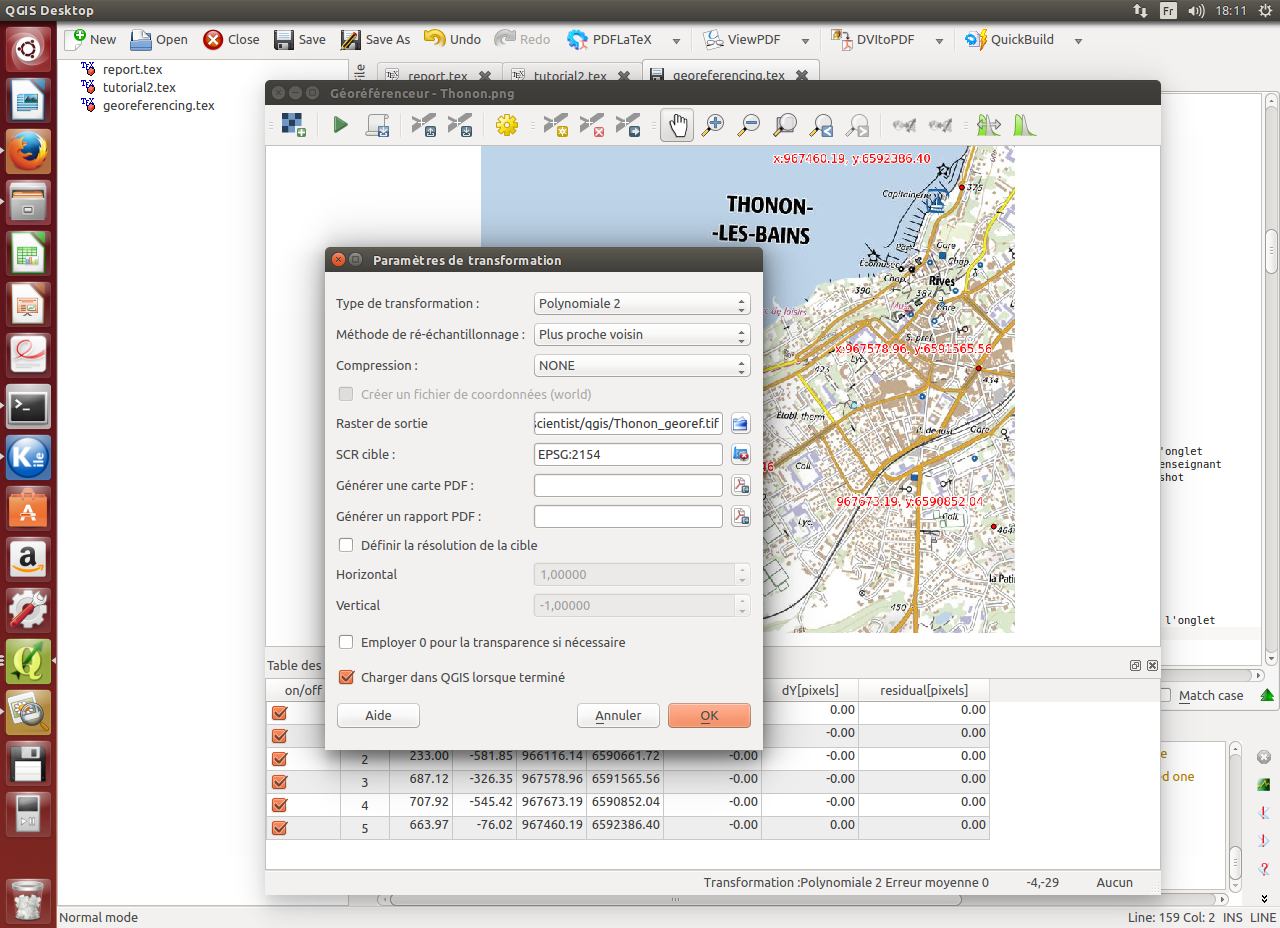
\includegraphics[scale=0.3]{images/qgis-transformation.png}
\end{center}
\caption{Projet $QGIS$ et renseignement de la transformation dans la fen\^{e}tre de géoréférencement}
\label{qgis-transformation}
\end{figure}

\clearpage

Il ne reste qu'à lancer la géoréférencement via la flèche verte dans la fen\^{e}tre de géoréférencement, cela va afficher
notre snapshot dans le système de coordonnées \begin{itshape}EPSG:32631\end{itshape} \ref{qgis-resultat}.

\begin{figure}[H]
\begin{center}
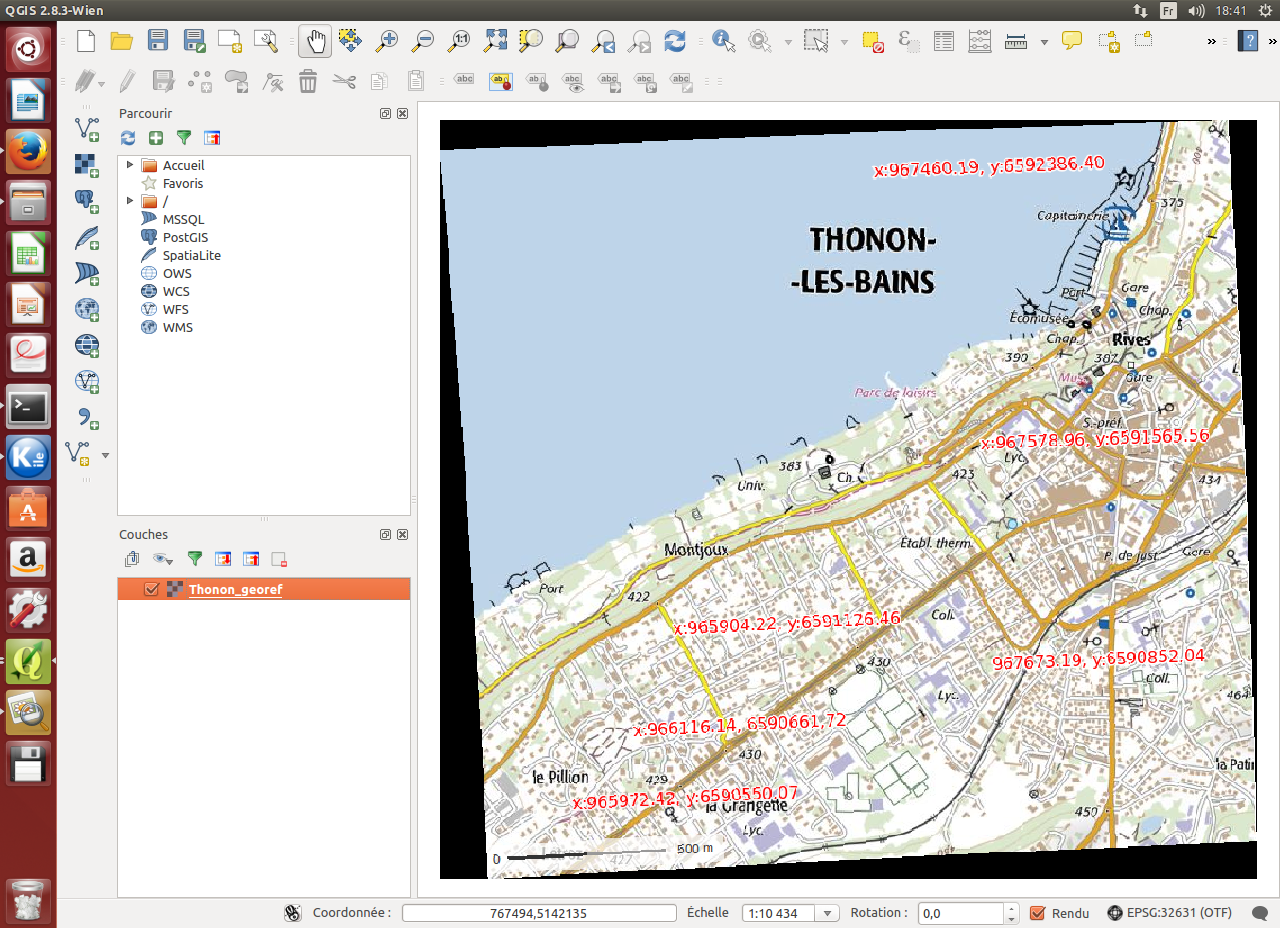
\includegraphics[scale=0.3]{images/qgis-resultat.png}
\end{center}
\caption{Projet $QGIS$ et affichage du raster géoéréférencé dans la fen\^{e}tre principale}
\label{qgis-resultat}
\end{figure}

\clearpage

\subsection{Superposition d'un raster Landsat-8}

A présent que notre snapshot IGN est géoréférencé et projeté dans le système de coordonnées de \begin{itshape}Landsat-8\end{itshape}
(\begin{itshape}EPSG:32631\end{itshape}), on peut charger une image géoréférencé \begin{itshape}Landsat-8\end{itshape} contenant la 
commune de \begin{itshape}Thonon-Les-Bains\end{itshape}. Pour cela, on a télécharger les bandes 2,3,4 correspondantes et formé l'image 
couleur  \ref{Thonon-landsat}.

\begin{figure}[H]
\begin{center}
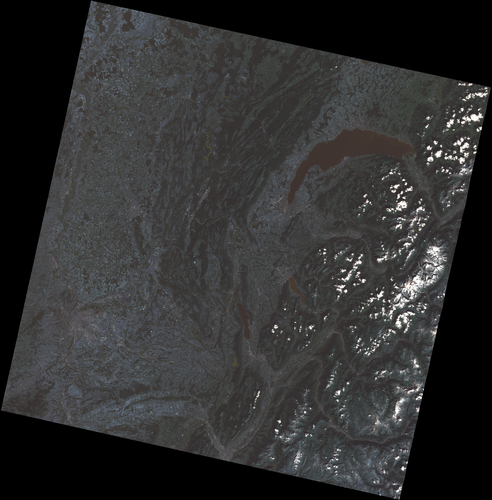
\includegraphics[scale=0.4]{images/Thonon_landsat.png}
\end{center}
\caption{Image couleur à partir d'images géoréférencées Landsat-8 contenant la commune de Thonon-Les-Bains}
\label{Thonon-landsat}
\end{figure}

On peut alors charger cette image dans la fenêtre principale $QGIS$ via l'onglet \og Couche > Ajouter une couche > Ajouter une couche 
raster \fg{}. On peut alors observer la superposition des deux rasters en réglant leur transparence (sous(fen\^{e}tre \og couches \fg{}) 
dans la fen\^{e}tre principale $QGIS$) \ref{qgis_super}

\begin{figure}[H]
\begin{center}
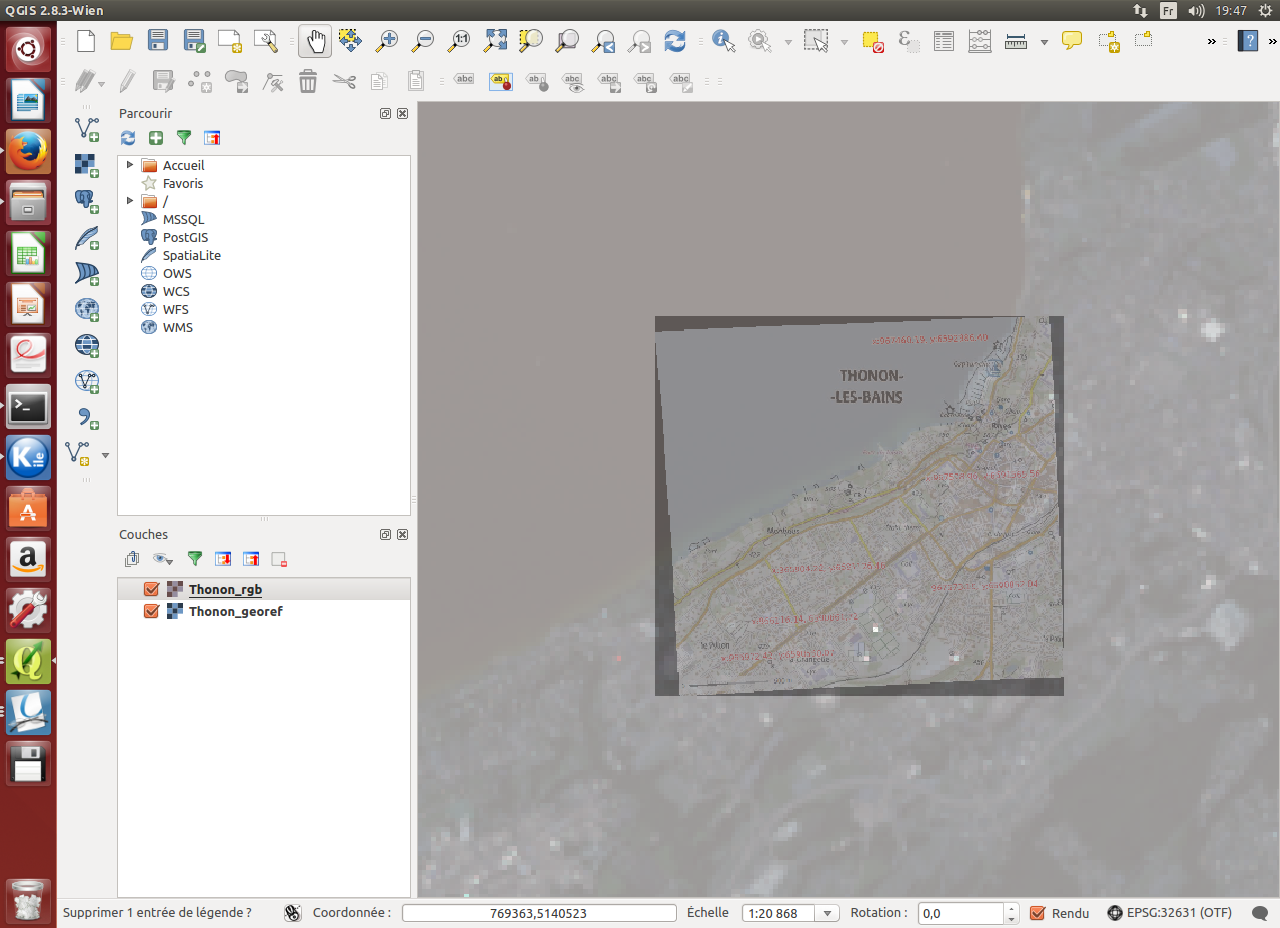
\includegraphics[scale=0.3]{images/qgis-superposition.png}
\end{center}
\caption{Projet $QGIS$ et superposition des rasters IGN et Landsat-8 géoréférencés en EPSG:32621 - commune de Thonon-Les-Bains}
\label{qgis_super}
\end{figure}

On constate une assez bonne superposition des deux rasters, le géoréférencement du satellite \begin{itshape}Landsat-8\end{itshape} peut
 donc \^{e}tre considéré comme convenable.
 
\clearpage

\backmatter

\listoftables

\listoffigures

\bibliographystyle{alpha}
\bibliography{biblio}

\end{document}